%\documentclass[11pt]{article}
%\usepackage{fullpage}

%\begin{document}

\subsection{Implementation plan}
The implementation of the TrackMe system will be done module by module and component by component. The order in which it is be carried out depends on a number of factors like the complexity of the modules and services, the dependence of other modules on the component being implemented and to the system as a whole, and it should also take into account the possibility of discovering flaws with the proposed design. If such an unfortunate event does happen, the flaws should be found and corrected as soon as possible, to limit the cost of the change of design. \newline

In this sense, the components of TrackMe, could be grouped in the following way, with the order specifying the order of implementation:
\begin{itemize}
\item[1.] Model
\item[2.] DataHandler and EmergencyManager
\item[3.] RunManager, NotificationManager, MapManager
\item[4.] UserManager and PaymentGateway
\end{itemize}

(note that by specifying the names of interfaces of components, we are also considering the concrete implementations, in which ever number they exist) \newline

The Model is proposed to be the first component that is implemented because all parts of the Application Server will be using some element of it and its role in allowing some service to communicate with the DBMSs in the Database Server component is crucial to the whole application. This also eliminates the possibility of every team and developer implementing a part of the Model on the fly, while implementing some service, which could lead to problems with integration and definitions of the same data concepts in different ways. \newline

The second group consists of the DataHandler and EmergencyManager components. They were identified as the most high risk part in the system and it would be advisable to focus on their implementation as soon as possible. They are singled out for the following reasons:

\begin{itemize}
\item DataHandler is one of the more complex components of the system, and it's the core of the entire application because it allows the app to support the Data4Help service. It has the most connections to any other part and so it has a vital role of grouping many functionalities of the system and providing
access to them to users. The implementation of this module is absolutely a primary concern.
\item EmergencyManager allows the app to support the AutomatedSOS service. It also interacts and depends on external services and components and even if its implementation is perhaps not the most complex, it is one of the high priority modules because the AutomatedSOS service is the one which has to guarantee the most high reliability and availability, so it's important to develop this module at the beginning, testing it a lot and eventually improve it in time.
\end{itemize}

The third group consists of the following:
\begin{itemize}
\item RunManager allows the app to support the Track4Run service, and it's one of the most complex modules of the system, even if it's not a primary concern because of the nature of the service itself (Data4Help and AutomatedSOS have a major importance in the general context of the application).
\item NotificationManager and MapManager heavily depend on external, already implemented services and components (not including the DBMS component). Because these components already exist, the parts of the system responsible with the task of communicating with them (the ones belonging to this group) have to be adapted to these external services. Although this fact has already been considered in the design of the system, this still represents a point of possible problems that require slight updates and changes to the
design. In that sense, their implementation should be done earlier than others.
\end{itemize}

Finally, the fourth group is composed by:
\begin{itemize}
\item UserManager, whose functions, while being some of the most crucial elements of the system, are CRUD operations that are relatively simpler than others that were already mentioned. Considering this, the component is not as risky as others because the time needed to complete it can be relatively accurately predicted.
\item PaymentGateway, that despite being a module which heavily depend on external systems, it's absolutely not crucial in the development of the application because payments are related just to some specific running races (not the main focus of the app).
\end{itemize}

\subsection{Integration and Testing}
\subsubsection{Entry criteria}

\subsubsection{Elements to be integrated}
The TrackMe system is composed of a number of components, as already shown, and the integration process can be grouped in the following way:
\begin{itemize}
\item Integration of components with DBMSs
\item Integration of components with (other) external services
\item Integration of components of the Application Server
\item Integration of the client (mobile application and wearable application) and the Application Server
\end{itemize}

\textbf{Integration of components with the DBMSs} - This group includes the integration of every part of the Application Server that uses the external server with the database, in any way (the "DBMS" notation refers to the external server with the database and its DBMSs). The specific integrations in this group are the following ones:
\begin{itemize}
\item[$\diamond$] UserManager, DBMS
\item[$\diamond$] DataHandler, DBMS
\item[$\diamond$] MapManager, DBMS
\item[$\diamond$] NotificationManager, DBMS
\item[$\diamond$] RunManager, DBMS
\end{itemize}

\textbf{Integration of components with the (other) external services} - In this group, we include the integration of every part of the system with an already existing and functional external service (without counting the DBMSs). They are the following ones:
\begin{itemize}
\item[$\diamond$] PaymentGateway, external Payment Gateway
\item[$\diamond$] MapManager, external Maps Provider
\item[$\diamond$] EmergencyManager, external SMS \& Voice Gateway
\item[$\diamond$] DataHandler, external Wearable Handler
\item[$\diamond$] NotificationManager, external Push Notifications Gateway
\end{itemize}

\textbf{Integration of the components of the Application Server} - Here, the integration between the parts of the Application Server is conducted. It is composed of:
\begin{itemize}
\item[$\diamond$] MapManager, RunManager
\item[$\diamond$] PaymentManager, RunManager
\item[$\diamond$] UserManager, RunManager
\item[$\diamond$] NotificationManager, RunManager
\item[$\diamond$] NotificationManager, UserManager
\item[$\diamond$] NotificationManager, DataHandler
\item[$\diamond$] DataHandler, EmergencyManager
\end{itemize}

\textbf{Integration of the client and the Application Server} - This is carried out to enable the sending of requests to the server via the mobile application (and interactions with the wearable application) which the user will be utilizing.

\subsubsection{Integration testing strategy}
The chosen strategy for the integration testing is the incremental integration testing, in particular the bottom-up one is the most suitable for the application. This allows us to start the integration and it’s testing while not waiting for the completion of the development and the unit testing of each component in the system. Considering the integration of two components, we would assume that, in best case, they have been implemented fully and that their respectful unit tests pass. However, the integration can, in some cases, start, if necessary, before the implementation has been completed. This can be allowed if the part of the component needed for that specific integration has been completed and tested. \newline

Since the opted solution is to start from the bottom-up, that means that the among the first integrations performed will have the already built external components in them. Since the application rests on these services and the communication with them, this order of integration and testing will enable the earlier detection of errors in these critical parts. \newline

It should be noted that it can be assumed that each integration in the same level of hierarchy (defined by the groups of integrations in the previous chapter) is independent and there is no specific order in
which to complete them. In this way, the integration process and its testing are more flexible. \newline

Finally, black-box testing is suitable for integration, system and acceptance testing. This kind of tests are perfect because they are specs-based and not code-based, and can help identifying missing functionalities in the system, so the idea is to begin with black-box tests as soon as possible.

\subsubsection{Sequence of component/function integration}
In this section, the list and order of every integration that is performed is shown. As already stated, the integration will be performed with the bottom-up strategy. As a notation used, the arrow pointing from the first component in the integration to the second means that the second one is using the services of the first component. \newline

It should be noted that there will be no explicit integration of the Model with any of the other components. This is because the nature of the component, the extent of the usage and dependency of other components on it and the implementation plan, that clearly states that the Model will be the first part that is implemented, mean that the integration itself is already being done during the implementation phase of the depending components and its correctness will inherently be tested by the unit tests of each component. \newline

It should also be noted, as stated before in this section, that the "DBMS" notation refers to the external server with the database and its DBMSs and that every "service" component considers all of the implementations, whatever they may be, of the specified interface. \newline

\paragraph{Integration of components with DBMSs}
\begin{center}
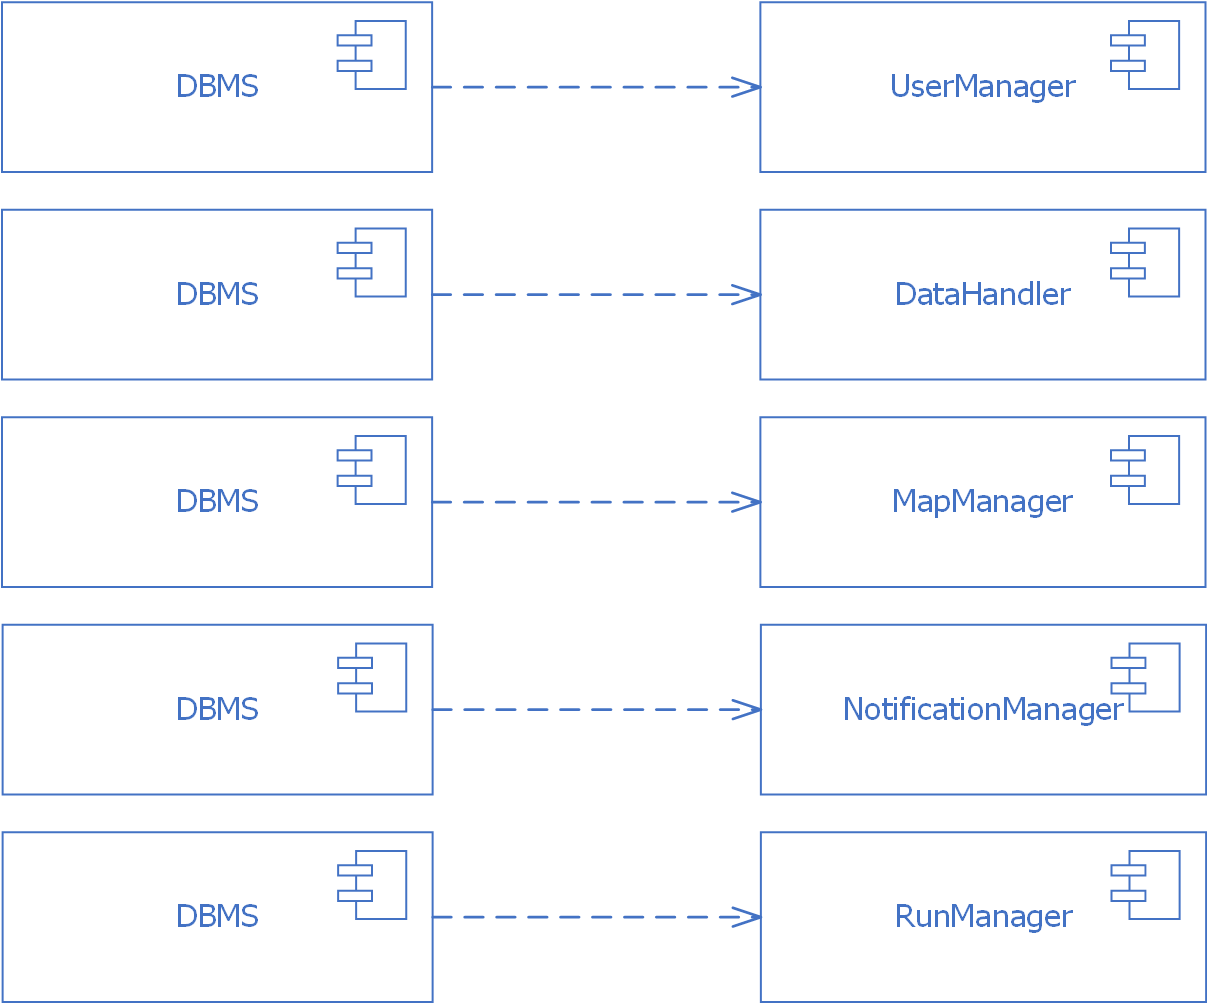
\includegraphics[scale=0.7]{sections/diagrams/integrationComp-DBMS.png}
\newline
\captionof{figure}{Integration of components with DBMSs. Each of the components shown here has the operations needed to work with the database, concerning the parts of the Model that they are using}
\end{center}

\paragraph{Integration of components with (other) external services}
\begin{center}
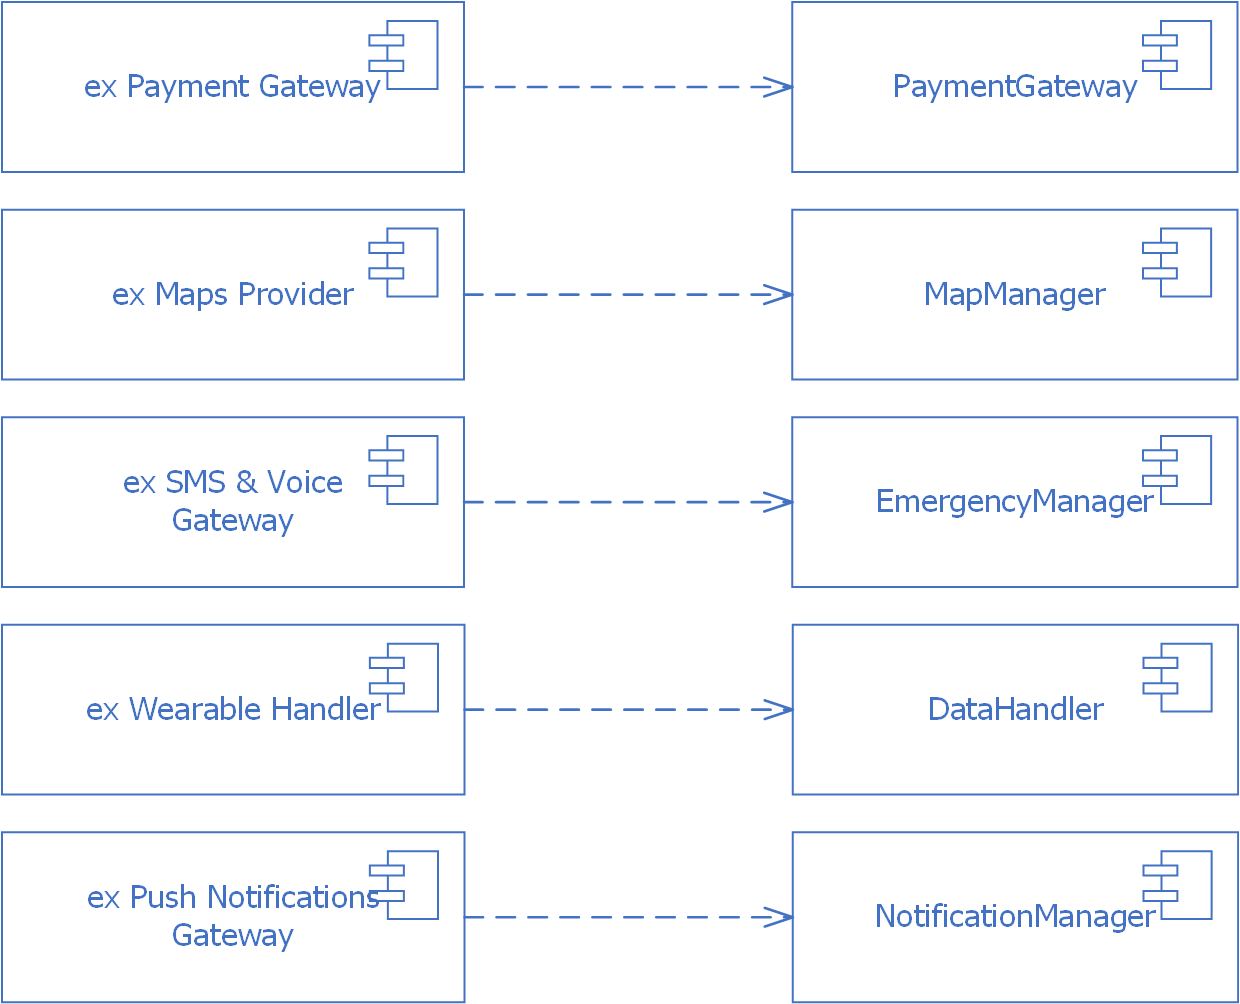
\includegraphics[scale=0.7]{sections/diagrams/integrationComp-ExComp.png}
\newline
\captionof{figure}{Integration of components with (other) external services. External service components, not considering the database, are integrated with either the components of the Application Server that dedicated to their usage them or the client mobile (or wearable) application}
\end{center}

\paragraph{Integration of components of the Application Server}
\begin{center}
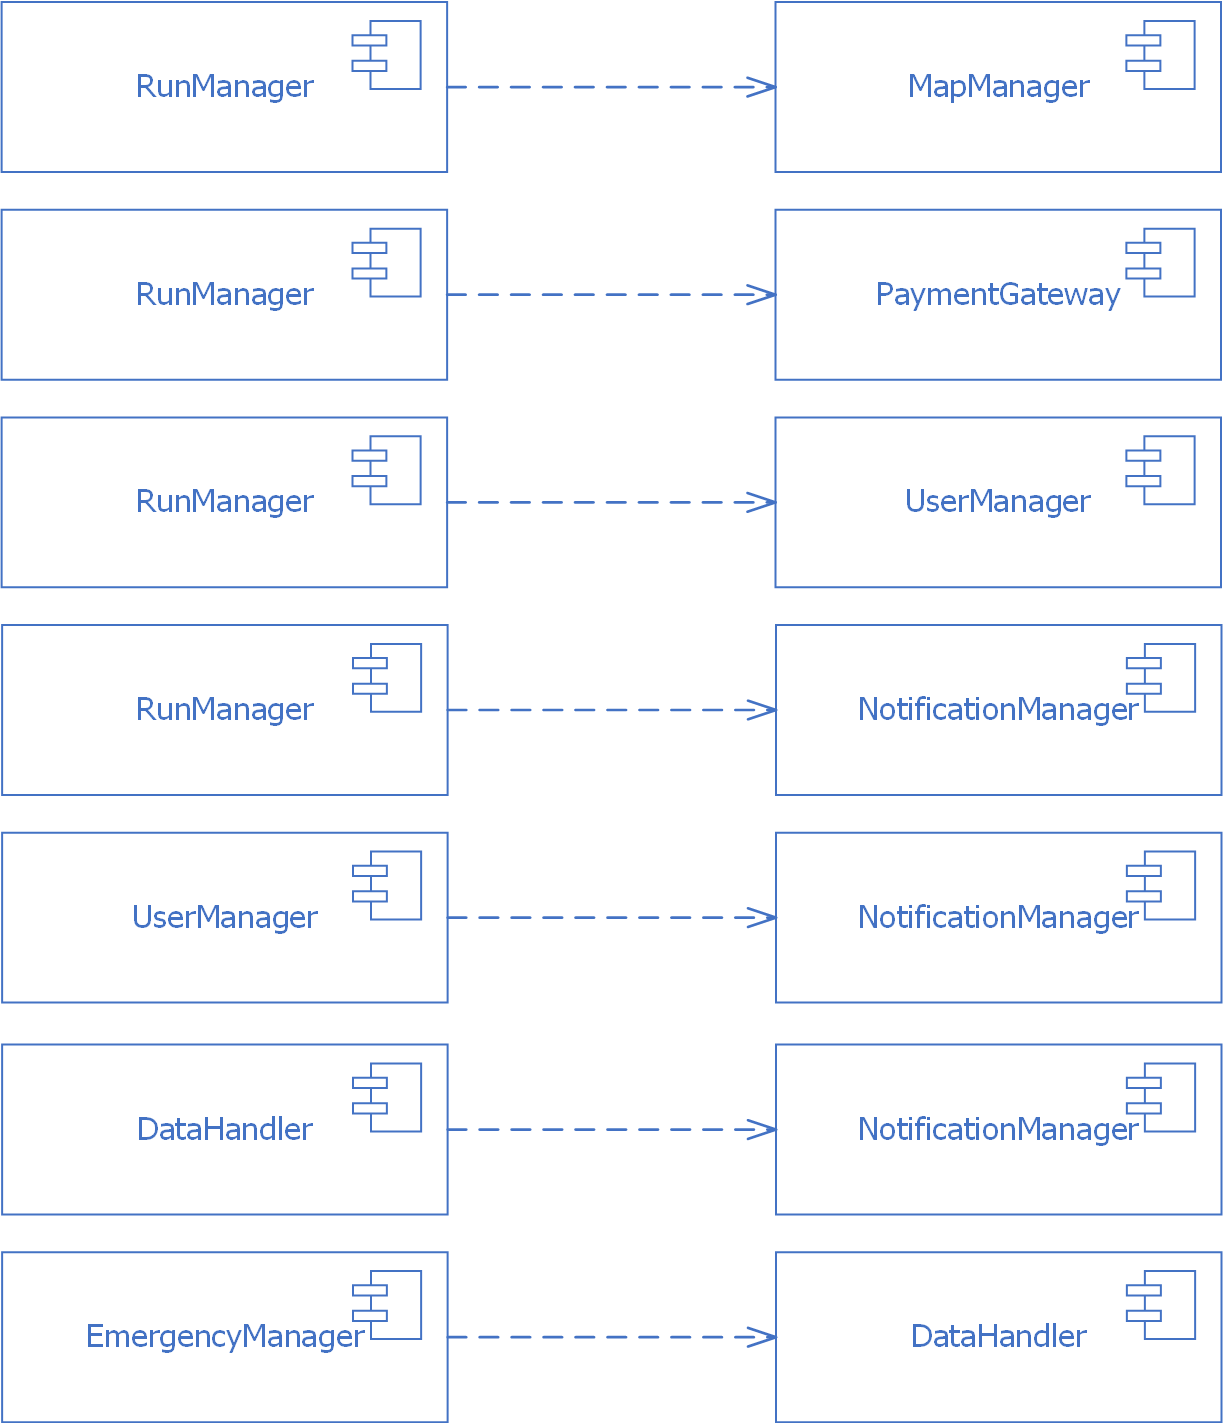
\includegraphics[scale=0.7]{sections/diagrams/integrationComp-Comp.png}
\newline
\captionof{figure}{Integration of components of the Application Server. After this phase of integration and testing is complete, the Application Server should be integrated fully, while being connected to the Database Server}
\end{center}

\paragraph{Integration of the client (mobile application and wearable application) and the Application Server}
\begin{center}
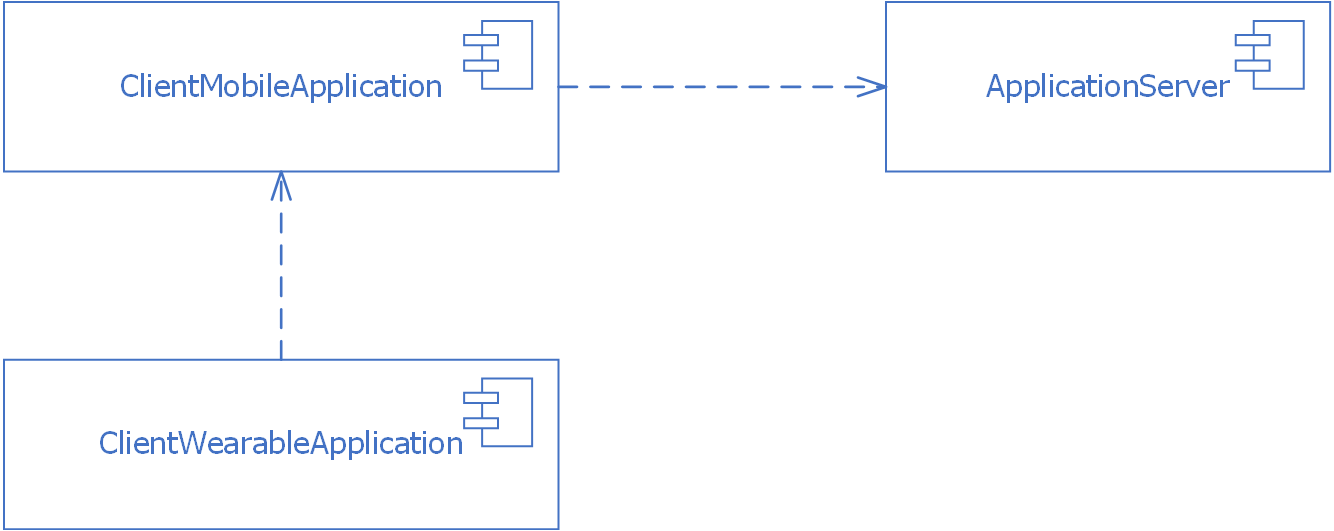
\includegraphics[scale=0.7]{sections/diagrams/integrationClient-AppServ.png}
\newline
\captionof{figure}{Integration of the client (mobile application and wearable application) and the Application Server. It should be done last, after at least most, if not all, of the Application Server parts have been developed and integrated}
\end{center}

%\end{document}